\subsection{Kaya Decomposition}

To understand the emissions of CO\textsubscript{2} of copper production Chili we need to decompose in more granular components in order to identify the technological and policy levers available to reduce CO\textsubscript{2} emissions from Chilean copper production. The decomposition is the following: 

\begin{equation}
\text{CO}_2 = \text{Ore} \times \frac{\text{prod}}{\text{Ore}} \times \frac{E_{\text{tot}}}{\text{prod}} \times \sum_{i} \left[ \frac{E_i}{E_{\text{tot}}} \times \left( \frac{E_{\text{comb},i}}{E_i} \cdot \text{CI}_{\text{comb,i}} + \frac{E_{\text{elec},i}}{E_i} \cdot \text{CI}_{\text{elec,i}} \right) \right]
\end{equation}

where $i \in \{\text{Open pit, Underground mining, Concentrating plant, Smelter, Electrolytic refining,}$\\
$\text{LX-SX-EW, Services}\}$
\\
To have a global view of the environmental impact the production cycle of copper we decided to look at the impact of each process along production chain. The sum over i decomposes the impact for every processes.
\\
\textbf{Production and ore processing:}
\begin{itemize}
    \item $\text{Ore}$ = Quantity of ore mined [kT], calculated as $\text{Ore} = \frac{\text{prod}}{\text{grade}}$
    \item $\text{prod}$ = Total copper production (cobre fino) [kT]
    \item $\frac{\text{prod}}{\text{Ore}}$ = Average Chilean ore grade [\%]
\end{itemize}

\textbf{Energy consumption:}
\begin{itemize}
    \item $\frac{E_{\text{tot}}}{\text{prod}}$ = Total energy intensity across all processes [MJ/kT copper]
    \item $\frac{E_i}{E_{\text{tot}}}$ = Share of total energy consumed by process $i$
    \item $E_{\text{tot}} = \sum_{i} E_i$ = Total energy consumption [MJ]
\end{itemize}

\textbf{Energy mix by process:}
\begin{itemize}
    \item $\frac{E_{\text{comb},i}}{E_i}$ = Fraction of combustion fuel energy in process $i$
    \item $\frac{E_{\text{elec},i}}{E_i}$ = Fraction of electricity in process $i$
    \item $E_i = E_{\text{comb},i} + E_{\text{elec},i}$ for each process $i$
\end{itemize}

\textbf{Carbon intensity:}
\begin{itemize}
    \item $\text{CI}_{\text{comb,i}} = \frac{\text{CO}_{2,\text{comb,i}}}{E_{\text{comb,i}}}$ = Carbon intensity of combustion fuels (direct emissions) in process $i$ [kT CO\textsubscript{2}/MJ]
    \item $\text{CI}_{\text{elec,i}} = \frac{\text{CO}_{2,\text{elec,i}}}{E_{\text{elec,i}}}$ = Carbon intensity of electricity (indirect emissions) in process $i$ [kT CO\textsubscript{2}/MJ]
\end{itemize}

Each ratio highlights a possible lever of action to reduce CO\textsubscript{2}, it can be a technological lever or a policy lever. At the same time we can analyze which are the main drivers of greenhouse emission due to copper production in Chili.
\subsection{Interpretation of components}
\textbf{Ore grade} is an important driver of impact because the density of copper in the ground varies and diminishes the deeper the mine is. It requires more energy and work, therefore more ore extracted, to get the same amount of copper produced. Ore grade has a direct impact on emissions. Moreover, ore grade is a variable that is not manageable by humans; it is a natural constraint that we will face by extracting more and more copper. Thus, it is very important to act on other levers to diminish the impact.
\\\\
\textbf{Total energy intensity} gives an important overview of how energy intensity evolved over the years. It doesn't give precise information about which process has the most impact or how their energy intensity changed, but it provides an overview of how the copper production chain's energy intensity has progressed.
\\\\
\textbf{Carbon intensity type by process} is very important to dig deeper into the decomposition and have a clearer and more precise view of which processes and which source of energy (either direct from fuel or indirect from electricity) are the most carbon intensive and where there is the most space for improvement. For carbon intensity from direct emissions, it is a good proxy of technological development, whether the machines and techniques used during the production process are more efficient and less polluting for the same energy consumption. On the other hand, for the use of indirect energy, the carbon intensity is also a good proxy to know how electricity is produced and what the principal sources are, whether they are renewable or not.
\\\\
\textbf{Fraction of energy type by process} is a crucial component of our decomposition and a lever to decarbonize the sector. As discussed in the paragraph above, technological improvement can have a great impact on carbon intensity for direct emissions; however, we can also see technological improvement as a shift from fuel usage to electricity. It is important to keep in mind that this shift is meaningful only if electricity production in Chile is also evolving toward sustainable production from renewable sources. We will discuss this in more detail later on.
\\\\
\textbf{Share of total energy by process} is a meaningful component because it gives a clear view of the importance of each process in the copper production cycle. Working on the emissions of the biggest processes is a much bigger lever on the impact due to their energy consumption. If the carbon intensity of a low energy consumption process is diminished, it would be much less impactful on emissions than improving a process with a high share of total energy consumption. Thus, it is very important to focus on the right processes.
\subsection{Components to TAP}
In the previous subsection, we have already given a first hint of how the components of the decomposition could be associated with technology, affluence, and population. Even though there is no population in this decomposition, the ore serves as it, because it represents all the rock extracted from the ground. Affluence in this decomposition represents the level of copper density in the ground, in other words, ore grade. The rest of the decomposition can be associated with technology. Since it is a Kaya decomposition, "technology" is broken down into two parts: energy intensity and carbon intensity. Furthermore, the decomposition breaks down carbon intensity by another level by looking at each process and at the source of energy, either direct (fuel) or indirect (electricity).
\subsection{Data Sources}
The data used to analyse this decomposition relies on one main source. The dataset used is published by COCHILCO (COMISIÓN CHILENA DEL COBRE), which is the Chilean commission of copper. The main mission of COCHILCO is to oversight the copper industry and advice the government so that this sector is preserved and can continue to develop in sustainable way.\cite{CochilcoWebsite2025} The Excel file with the data used and plenty of other data can be found on there website under publications (publicaciones) and then under sustainability (sustentabilidad). The dataset used goes from 2015 to 2024. \footnote{https://www.cochilco.cl/web/\#}
\subsection{Evolution of CO$_2$ drivers in copper production}

\begin{figure}[H]
    \centering
    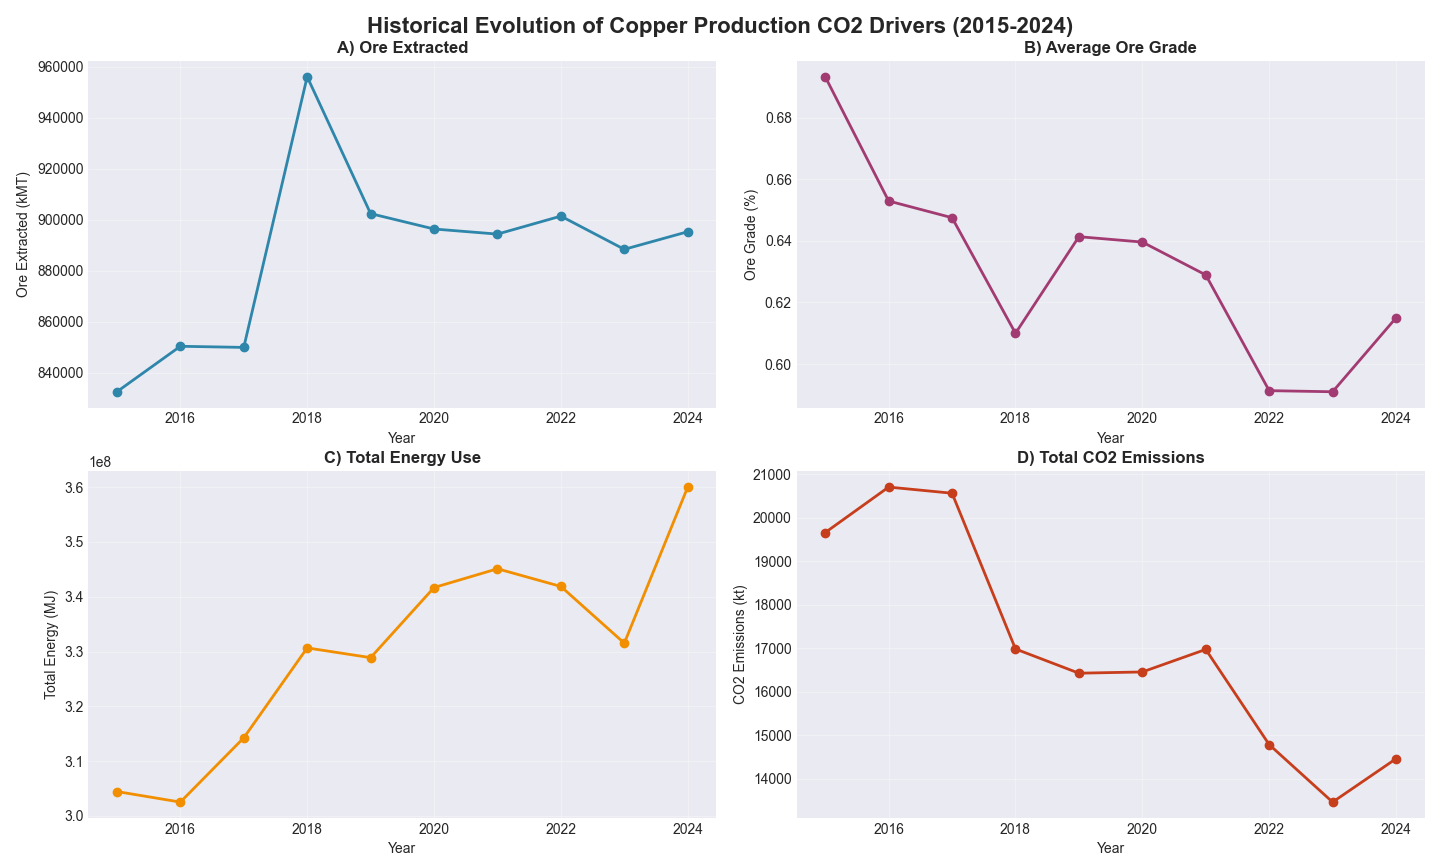
\includegraphics[width=0.9\linewidth]{Figures/Figure_1.png}
    \caption{Historical Evolution of Copper Production CO2 Drivers (2015-2024)}
    \label{fig:cen_region}
\end{figure}
\textbf{Panel A:} shows the evolution of ore extracted in metric tonnes. Between 2017 and 2018 we see a very high increase but then on a stabilization around 900'000 kT. 
\\\\
\textbf{Panel B:} highlights how the average ore grade of copper evolved over the years. We can clearly see a downward trend with a decrease higher than 10\% over ten years. Years where ore grade improved (2019 and 2024) were probably due to the discovery of new reserves with higher copper concentration in the ground.
\\\\
\textbf{Panel C:} displays how total energy consumption during the production cycle evolved between 2015 and 2024. The upward trend is clear, with more than a 15\% increase in energy consumption. This increase can clearly be associated with the decrease in ore grade, which translates into much more rock extraction from the ground. Between 2020 and 2022, energy consumption stabilized during years when production also decreased, suggesting a direct link between production volume and energy use.
\\\\
\textbf{Panel D:} tracks the total amount of greenhouse gas emissions due to copper production. Over the years, there has been a constant downward trend with a decrease of one third. While energy consumption increased, this suggests that important improvements have been made to limit CO$_2$ emissions over the last ten years. 
\\\\
These four figures highlight that the amount of ore extracted has been quite constant over years (apart from a peak in 2018), while ore grade clearly had a downward trend and energy consumption an upward trend. Because ore extracted has been quite constant in the previous year while ore grade declined, it suggests that production of copper has also a bit declined. The most important point is to see that overall, the total amount of CO$_2$ emissions has decreased by more than 20\%, showing that progress has been made and can continue to be made. In the next sections, we will try to dig deeper and explore in more detail what are the causes and reasons for this decline and what can still be done to reduce the impact of copper production in Chile. As discussed in section \ref{sec:evol of mining energy}, the scale and growing complexity of production has increased the total energy consumption.
\subsection{Carbon Intensity and Electrification Indicators}
\begin{figure}[H]
    \centering
    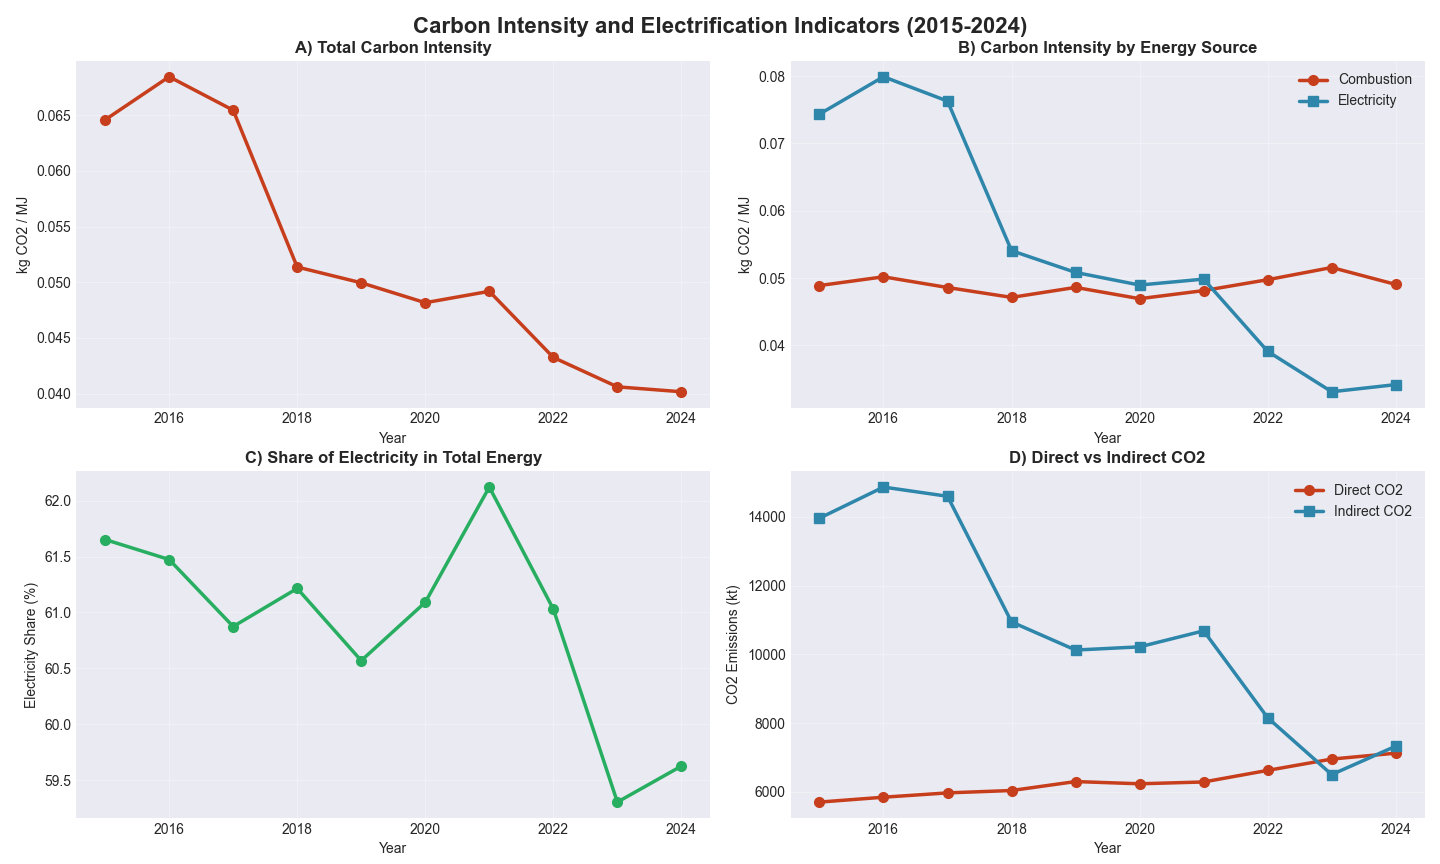
\includegraphics[width=0.9\linewidth]{Figures/Figure_2.png}
    \caption{Carbon Intensity and Electrification Indicators (2015-2024)}
    \label{fig:cen_region}
\end{figure}
\textbf{Panel A:} shows how carbon intensity evolved over the years. In this case, it is the total carbon intensity and it is not decomposed between direct and indirect carbon intensity. Over the years, there is a downward trend, with a total decrease of around one-third.
\\\\
\textbf{Panel B:} compares the evolution of carbon intensity from direct use of energy (fuel) and indirect use of energy (electricity). The carbon intensity from direct emissions stays constant over the years, while the carbon intensity from electricity has decreased by half over the last ten years. This suggests that overall, machines or processes using fuel have not evolved much in terms of efficiency, while the production of electricity used in copper production has diminished its impact considerably.
\\\\
\textbf{Panel C:} displays the evolution of the electricity share in energy use. There has been a small downward trend between 2021 and 2024, but overall the share of electricity remained constant at around 61\%.
\\\\
\textbf{Panel D:} highlights the variation of direct and indirect CO$_2$ emissions. Direct emissions increased by approximately 10\%, while indirect emissions decreased by more than 50\%. Indirect emissions used to be the largest driver of total emissions, this is consistent with what has been discussed and highlighted in section \ref{sec:elec and CI}. This suggests that the decrease over the years in greenhouse gas emissions is mostly due to the decrease in emissions coming from electricity use. 
\\\\
These four figures highlight how the reduction in carbon intensity of electricity production in Chile has helped to decrease emissions in the copper production chain toward more sustainable sources. They also suggest that in terms of technical evolution of machines using fuel, overall their emissions didn't improve since the carbon intensity remained quite constant. On the other hand, the electricity share didn't evolve much either, strongly suggesting that the decrease in CO$_2$ is probably mainly due to the improvement of carbon intensity in electricity production. This highlights that Chile's renewable energy transition has been the primary driver of emissions reduction in the copper sector, rather than improvements in mining technology itself. We will explore the carbon intensity (direct and indirect) of the different processes and look at which have possible improvements and how they evolved over the years.
\subsection{Identify Key Drivers of CO2}
\begin{figure}[h]
    \centering

    \begin{subfigure}{0.7\textwidth}
        \centering
        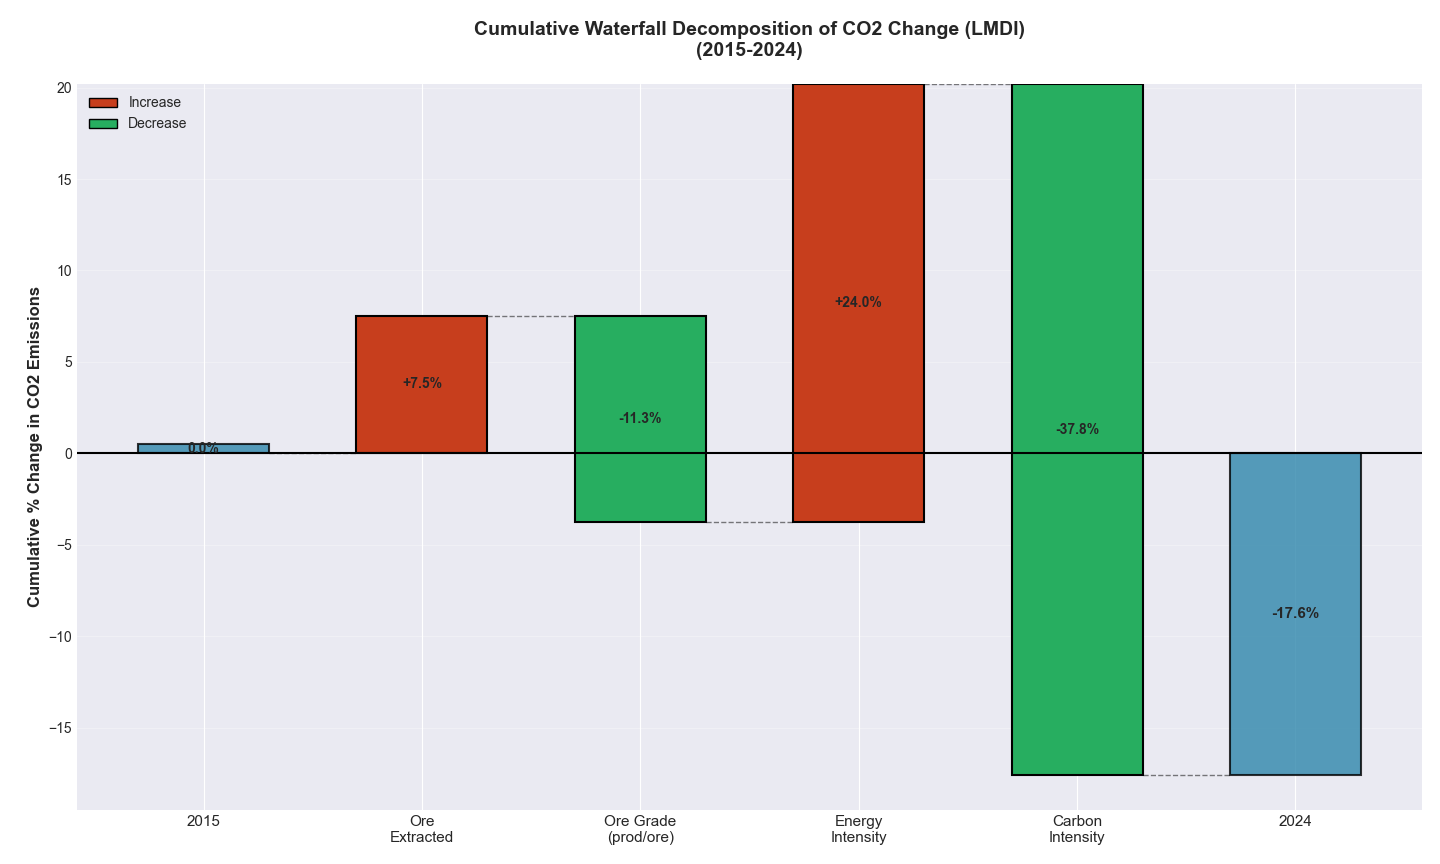
\includegraphics[width=\linewidth]{Figures/Figure_3.png}
        \caption{Cumulative Waterfall Decomposition of CO2 (LMDI)}
    \end{subfigure}
    \begin{subfigure}{0.7\textwidth}
        \centering
        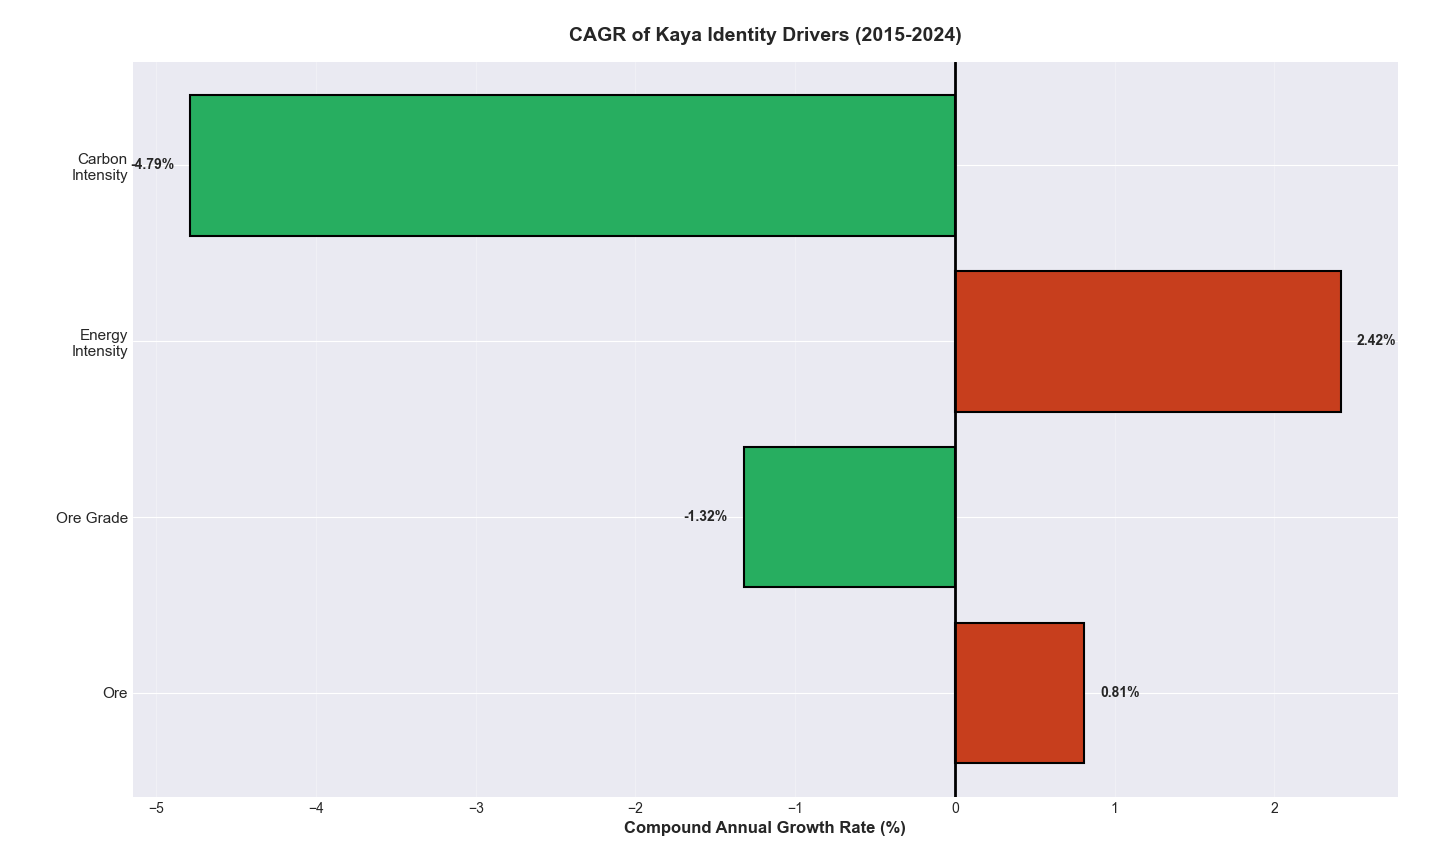
\includegraphics[width=\linewidth]{Figures/Figure_5.png}
        \caption{CGAR of Kaya Identity Drivers}
    \end{subfigure}
\end{figure}
\label{fig:waterfall}
The first figure is a waterfall chart that distributes the change in CO$_2$ emissions from copper production across the four components of the Kaya Identity using the LMDI method, while the second figure shows the compounded growth rate of the different Kaya Identity drivers. In the Kaya decomposition introduced earlier, carbon intensity corresponds to the aggregate contribution of all processes.

The combined effect of the growth in ore extraction and the decline in ore grade equals the growth rate in copper production between 2015 and 2024 (\textbf{7.5\% - 11.3\% = -3.8\%}), indicating that copper production declined over the period. This suggests that, although the quantity of ore extracted increased, it was not sufficient to offset the sharp decline in ore grade, resulting in a negative contribution to CO$_2$ emissions. This is also visible in the second figure, where the compounded growth rate of ore grade outpaces the growth rate of ore extraction.

Although energy intensity increased by \textbf{24\%}, total greenhouse gas emissions decreased over the years. This represents an absolute decoupling, driven primarily by the \textbf{37.8\%} reduction in carbon intensity. This is also visible in the CAGR graph, where the decline in carbon intensity (\textbf{-4.79\%}) outweighs the increase in energy intensity (\textbf{2.42\%}). These two charts therefore confirm the previous discussion: grid decarbonization was the main factor behind the decline in CO$_2$ emissions.


\subsection{Energy intensity and energy mix by process}
\begin{figure}[H]
    \centering
    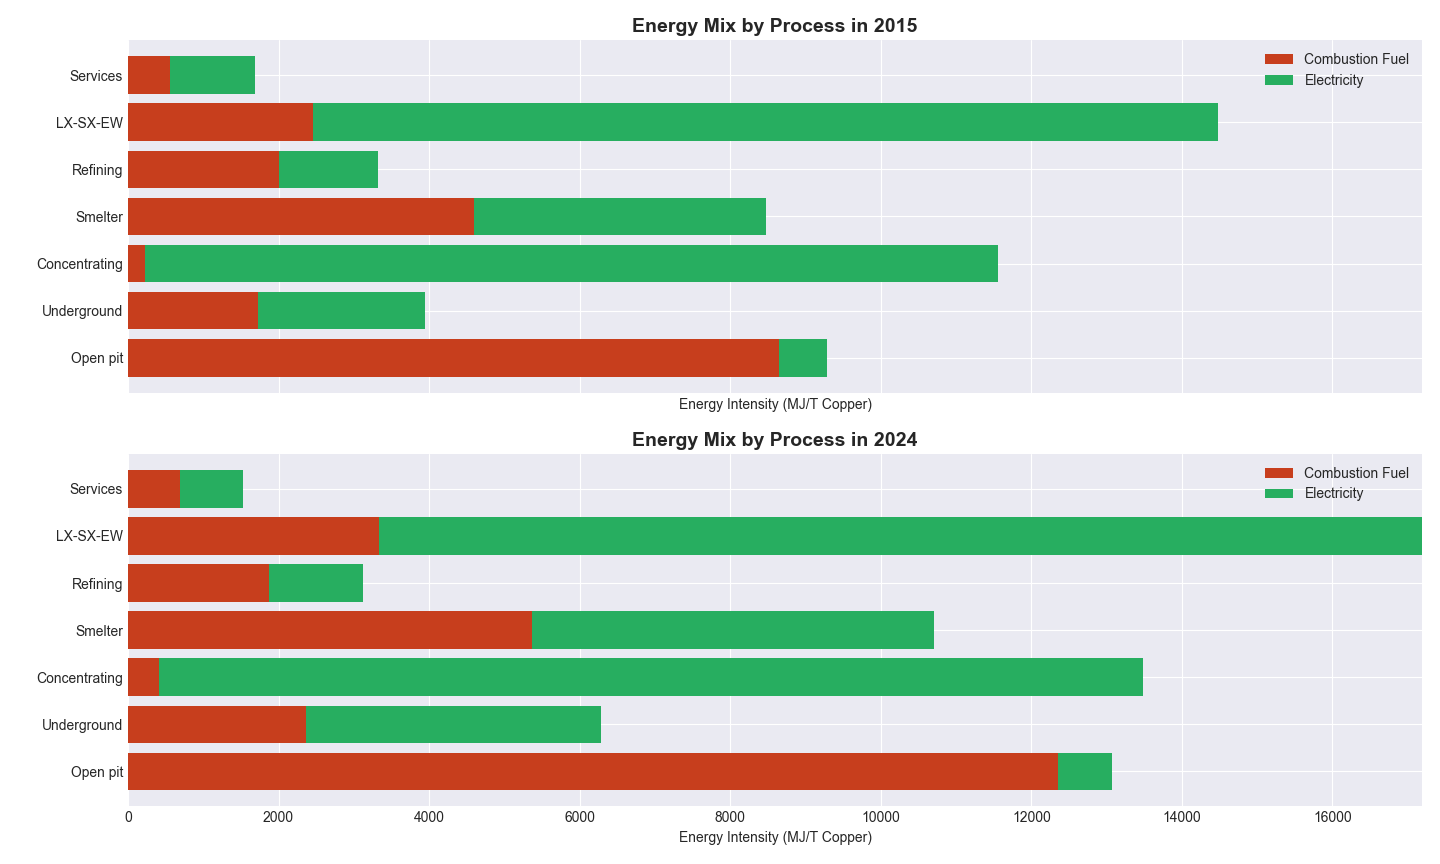
\includegraphics[width=1\linewidth]{Figures/Figure_4.png}
    \caption{Energy intensity and energy mix by process by process)}
    \label{fig:cen_region}
\end{figure}
This graph shows the total energy intensity, as well as its decomposition into direct and indirect energy intensity for each process in 2015 and 2024. We can clearly see that the activities related to the mining of copper (open pit and underground) are the most energy intensive and consume the most fuel energy. This suggests that much of the mining, especially open pit mining, is done with fuel combustion machines. LX-SX-EW is the second most energy intensive process, with a very large portion coming from electricity use due to electrowinning, where electric current drives the reduction of copper ions to metal. This once again demonstrates the importance of grid decarbonization. Apart from services and refining, every process increased its energy intensity, which is consistent with the increase in energy intensity seen in Figure \ref{fig:waterfall}.
\\
We can also remark that the share of electricity seems to stay approximately constant over the period, which suggests once again that the decrease in carbon intensity and therefore in greenhouse gas emissions is mainly due to grid decarbonization. We can also note that the overall electricity share of only \textbf{60\%} is mainly due to the open-pit mining process. Excluding open-pit mining, the share of electricity in total energy consumption would be significantly higher, since electricity represents a much larger proportion of energy use in the other processes. This is consistent with what was discussed in Section \ref{sec:global climate commitments}, where Chile has committed to achieving carbon neutrality by 2050 and to progressively phasing out coal-fired electricity generation.
\\
Even though carbon intensity has tumbled, there is still some room for improvement by decreasing the use of fuel energy in processes, especially in open pit mining and the smelter process. Later on, we will dedicate a section to understanding what are the possible improvements and electricity shifting opportunities. It is very important to mention that a shift toward more electricity use is beneficial only if there is continuous grid decarbonization.
\subsection{CO$_2$ emissions by process}
\label{sec:emissions by process}
\begin{figure}[H]
    \centering
    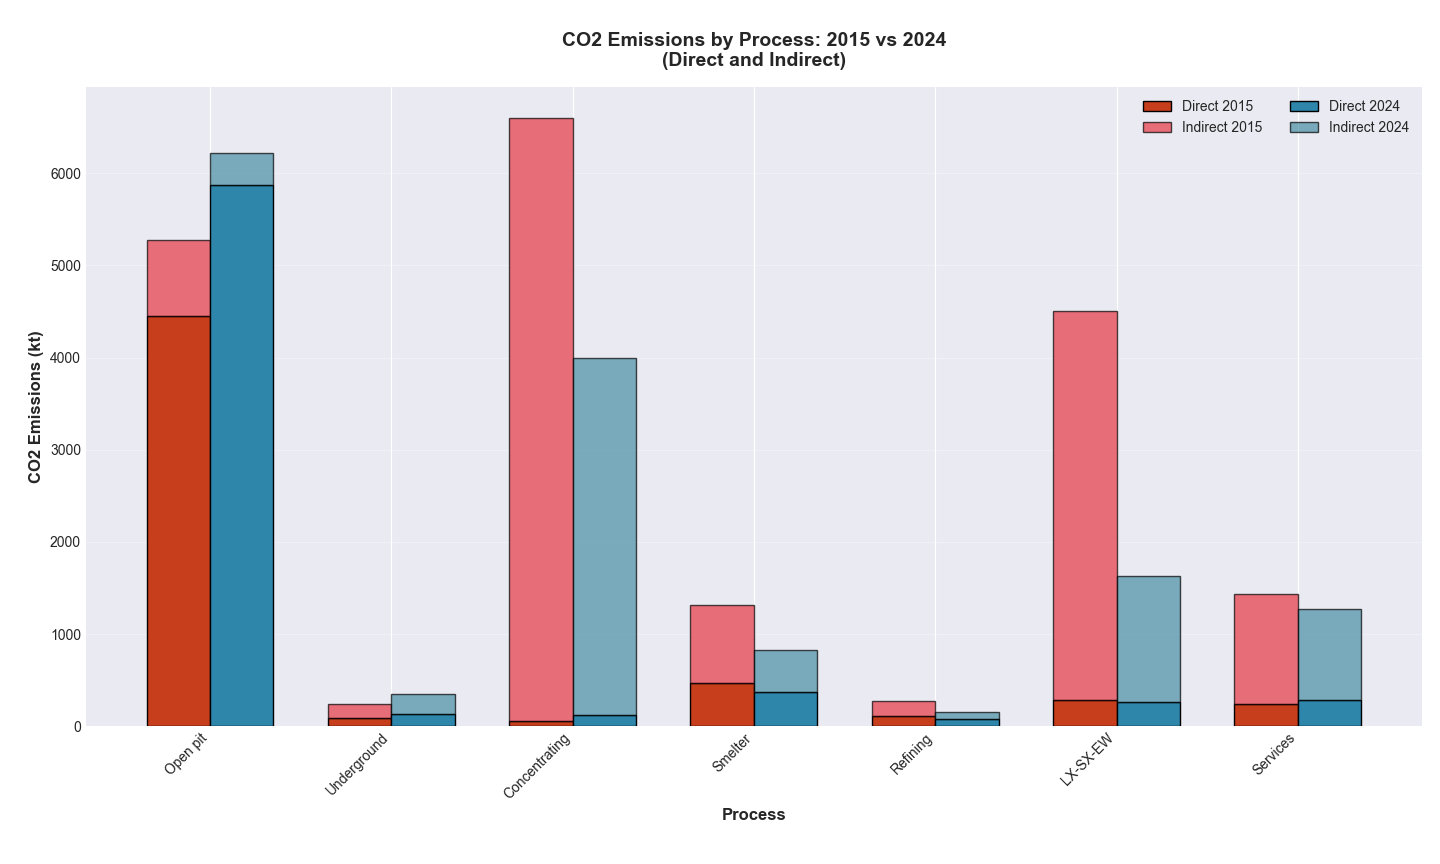
\includegraphics[width=0.9\linewidth]{Figures/Figure_6.png}
    \caption{CO$_2$ emissions by process (2015 vs 2024)}
\end{figure}
This figure compares greenhouse gas emissions for each process and decomposes them into direct emissions (fuel combustion) and indirect emissions (electricity consumption). It is clear that the most polluting processes are open-pit mining, concentrating, and the LX-SX-EW process. Apart from open-pit mining, the share of emissions originating from fuel combustion has remained relatively constant over the years, while emissions associated with electricity consumption have decreased significantly, particularly for concentrating and LX-SX-EW. The graph clearly shows that open-pit mining has a major impact on total emissions. Unlike the other processes, its emissions have increased rather than decreased over time. This is mainly because it is the only process in which fuel consumption represents a very large share of total energy use. These results suggest that electrifying open-pit mining activities, or reducing reliance on fuel intensive machinery, could represent one of the most effective levers for decarbonizing the copper production sector. From a broader perspective, each process has a distinct impact on total emissions, and the balance between direct and indirect emissions varies significantly across processes. As discussed in Section \ref{sec:heterogeneity}, emissions are highly heterogeneous throughout the production chain, making it essential to analyze each process separately.
\subsection{Opportunities for Decarbonization}
\label{sec:opportunities}
From the different figures that we have analyzed above, we have seen that CO$_2$ has decreased mainly due to grid decarbonization, which clearly relies on the fact that renewable sources represented nearly 70\% of Chile's electricity generation (Section \ref{sec:elec & renew}). It is thus very important that Chile continues to transition toward renewable resources.
\
As mentioned in Section \ref{sec:emissions by process}, the main lever to reduce CO$_2$ emissions is working on how to replace current machinery. Loading and hauling are among the major sources of greenhouse gas emissions in open-pit mining, so shifting from fuel-based transportation methods to electricity-based ones can be very impactful.
\
Therefore, replacing fuel haul-trucks with battery-electric or electric road system trucks can reduce CO$_2$ emissions significantly. Electric road systems are similar to trolley buses, meaning that trucks are powered by overhead lines. A simulation study by \textit{Lindgren et al., 2022} examined the feasibility of large battery-electric haul trucks using Aitik copper mine in Sweden. They concluded that compared to classic operation, electric haul trucks could increase productivity by 16\% while reducing costs by 44\%. \cite{Simulations_of_Battery_Electric} This suggests that apart from an environmental perspective, shifting toward electrified trucks also has economic value, which is very important because it increases the likelihood that large mining companies will invest in these technologies.
\
We also wanted to look concretely at what types of solutions are available on the market to decarbonize the sector. Liebherr, a Swiss equipment manufacturer, operates diesel-electric haul trucks equipped with the Trolley Assist System (Liebherr T 284) in the open pit of Collahuasi and has installed a 1 km trolley line. This results in a 26\% decrease in fuel consumption and a 94\% decrease in CO$_2$ emissions on the ramp. The company also offers electric mining excavators. They are also developing trucks with battery-electric powertrains and trucks operating with alternative fuels such as ammonia and hydrogen.\cite{Liebherr} However, loading and hauling represent more than 50\% of total mine input costs. This suggests that moving toward new machinery is very expensive and a complete fleet cannot be replaced easily.\cite{Mining_fleet_management}